\documentclass[UTF8]{beamer}
\usepackage{ctex}
\usepackage{graphicx}
\usepackage{ulem}
\usepackage{hyperref}
\usepackage{listings}
\usepackage{graphicx}

\usetheme[block=fill, sectionpage=none]{Berlin}
\usecolortheme{custom}

\title{组合数学}
\author{God\_Max\_Me}
\institute{Chengdu No.7 High School.}
\date{2025 年}
\usefonttheme[onlymath]{serif}

\geometry{paperheight=11.0cm,paperwidth=16.0cm}




\begin{document}
  \maketitle
  \section{前言}

    \begin{frame}{一些必要 trick}
      \begin{itemize}
        \item
          推式子,先提 $\sum$ 和 $\Pi$
          到最前面,然后从后往前合并,必要时考虑更改 $\sum$ 的取值
        \item
          看到次方变为斯特林数,$x^n=\sum\limits_{i=0}^{n} {n \brack i} {x \choose i}i!=\sum\limits_{i=0}^{n}\sum\limits_{i=1}^m{(-1)^{m-i}{i^n \over (m-i)!}}{x \choose i}$
        \item
          注意莫反、欧反的形式
      \end{itemize}
    \end{frame}

    \begin{frame}{推式子基本原理}
      \begin{itemize}
        \item
          先把 $\sum$ 移到最前面。
        \item
          将多个 $\sum$ 排序,范围更小的放在前面。
        \item
          将只与当前 $\sum$ 有关的式子尽量往前提。
        \item
          将能简化式子的特殊边界提出来。
        \item
          从后往前处理。
      \end{itemize}
    \end{frame}
    
  \section{组合数学}
  \subsection{组合恒等式}

    \begin{frame}
      \begin{block}{递推式}
        $$
        {n \choose m}={n-1 \choose m}+{n-1 \choose m-1}
        $$
      \end{block}
      
      \pause
      证明

      从组合意义上推导,在 $n$ 个人中选 $m$
      个相当于单独考虑最后一人,若他要选,则为 ${n-1 \choose m-1}$ 他不选则为
      ${n-1 \choose m}$。
    \end{frame}
    
    \begin{frame}
      \begin{block}{吸引/相伴等式}
        $$
        \begin{aligned}
        {{n \choose m} \over {n-1 \choose m-1}}&={{n} \over {m}} \\
        {{n \choose m} \over {n-1 \choose m}}&={{n} \over {n-m}} \\
        {{n \choose m} \over {n \choose m-1}}&={{n-m+1} \over {m}} \\
        \end{aligned}
        $$

        \pause
        另外的形式:

        $$
        \begin{aligned}
        k {n \choose k}&=n {n-1 \choose k-1} \\
        (n-k){n \choose k}&=n{n-1 \choose k}
        \end{aligned}
        $$
      \end{block}
    \end{frame}

    \begin{frame}
      \begin{block}{上指标反转}
        $$
        {n \choose m}=(-1)^m{m-n-1 \choose m}
        $$
      \end{block}
      \pause
      证明

      $$
      \begin{aligned}
      {n \choose m}={n^{\underline{m}} \over m!}&={n\times(n-1)\times (n-2)\times...\times (n-m+1) \over m!} \\
      &={(-1)^m\times (-n)\times(1-n)\times...\times(m-n-1) \over m!} \\
      &={(-1)^m\times (m-n-1)^{\underline{m}} \over m!} \\
      &=(-1)^m{m-n-1 \choose m}
      \end{aligned}
      $$
    \end{frame}

    \begin{frame}
      \begin{block}{三项式系数恒等式}
        $$
        {n \choose m}{m \choose k}={n \choose k}{n-k \choose m-k}
        $$

        等式两边拆开约分即可得证。
      \end{block}
      \pause
      \begin{block}{平行求和}
        $$
        \begin{aligned}
        {n \choose 0}&+{n+1 \choose 1}+...+{n+m \choose m} \\
        &=\sum\limits_{i=0}^{m}{n+i \choose i}={n+m+1 \choose m} \\
        m &\in \mathbb{N}
        \end{aligned}
        $$
        \pause
        证明

        将${n+m+1 \choose m}$用加法公式展开即可。
      \end{block}
    \end{frame}

    \begin{frame}
      \begin{block}{上指标求和}
        $$
        \sum\limits_{i=0}^{n}{i \choose m}={n+1 \choose m+1}
        $$
        \pause
        证明

        从组合意义入手,相当于我从 \(n+1\) 个数中选 \(m+1\) 个数,先假设选
        \(i\),那么 \(i\) 前面还需要选 \(m\) 个数,枚举这个 \(i\),即为答案。
        也可通过微积分求导知识进行证明,这里不再详述。
      \end{block}
    \end{frame}

    \begin{frame}
      \begin{block}{练习一:}
        求 \(\sum\limits_{i=0}^{m}{n+i \choose i}\)
      \end{block}
      \pause
      解
      \[
      \begin{aligned}
        \sum\limits_{i=0}^{m}{n+i \choose i}&=\sum\limits_{i=0}^{m}{n+i \choose n+i-i} \\
        &=\sum\limits_{i=0}^{m}{n+i \choose n} \\
        &={n+m+1 \choose n+1}
      \end{aligned}
      \]
    \end{frame}

    \begin{frame}
      \begin{block}{下指标求和(整行)}
        \[
        \sum\limits_{i=0}^{n}{n \choose i}=2^n
        \]
      \end{block}
      \pause
      证明
      \[
      \begin{aligned}
        \sum\limits_{i=0}^{n}{n \choose i}&=\sum\limits_{i=0}^{n}{n \choose i}1^{n-i}1^i \\
        &=(1+1)^n=2^n
      \end{aligned}
      \]
      \pause
      \begin{block}{交错求和}
        \[
        \sum\limits_{k=0}^{m}(-1)^k{n \choose k}=(-1)^m{n-1 \choose m},m\in \mathbb{Z}
        \] 
      \end{block}
    \end{frame}

    \begin{frame}
      证明
      \[
      \begin{aligned}
        \sum\limits_{k=0}^{m}(-1)^k{n \choose k}&=\sum\limits_{k=0}^{m}{k-n-1 \choose k} \text{上指标反转} \\
        &={m-n \choose m}  \text{平行求和} \\
        &=(-1)^m{n-1 \choose m} \text{上指标反转}
      \end{aligned}
      \]
      \pause
      \begin{block}{下指标卷积(范德蒙德卷积)}\label{ux4e0bux6307ux6807ux5377ux79efux8303ux5fb7ux8499ux5fb7ux5377ux79ef}
      \[
      \sum\limits_{i=0}^k{n \choose i}{m \choose k-i}={n+m \choose k}
      \]
      \end{block}
      \pause
      证明

      从 \(n\) 个数中选 \(i\) 个数,再从 \(m\) 个数中选 \(k-i\) 个数,相当于从
      \(n+m\) 个数中选 \(k\) 个数。
    \end{frame}

    \begin{frame}
      \begin{block}{练习二:}\label{ux7ec3ux4e60ux4e8c}
      求 \(\sum\limits_{i=0}^{m}{n \choose i}{m \choose i}\)
      \end{block}
      \pause
      解

      \[
      \begin{aligned}
      \sum\limits_{i=0}^{m}{n \choose i}{m \choose i}&=\sum\limits_{i=0}^{m}{n \choose i}{m \choose m-i} \\
      &={n+m \choose m}
      \end{aligned}
      \]
    \end{frame}

    \begin{frame}
      \begin{block}{上指标卷积}\label{ux4e0aux6307ux6807ux5377ux79ef}
      \[
      \sum\limits_{i=0}^{n}{i \choose a}{n-i \choose b}={n+1 \choose a+b+1}
      \]
      \end{block}
      \pause
      证明
      相当于从左边 \(i\) 个中选 \(a\) 个,右边 \(n-i\) 个中选 \(b\) 个。等于从
      \(n\) 个中选 \(a+b\) 个,枚举分割点 \(i\)。
    \end{frame}
    \begin{frame}
      \begin{block}{练习三:}\label{ux7ec3ux4e60ux4e09}
      求 \(\sum\limits_{i=m}^{n}(-1)^i{n \choose i}{i \choose m}\)
      \end{block}
      \vspace{-1em}
      \pause
      \[
      \begin{aligned}
      \sum\limits_{i=m}^{n}(-1)^i{n \choose i}{i \choose m}&=\sum\limits_{i=m}^{n}(-1)^i{n \choose m}{n-m \choose i-m} \\
      &={n \choose m}\sum\limits_{i=m}^{n}(-1)^i{n-m \choose i-m} \\
      &={n \choose m}\sum\limits_{i=0}^{n-m}(-1)^{i+m}{n-m \choose i} \\
      &={n \choose m}(-1)^m\sum\limits_{i=0}^{n-m}(-1)^{i}{n-m \choose i}\times 1^{n-m-i} \\
      &={n \choose m}(-1)^m 0^{n-m}=(-1)^m[n=m] \\
      \end{aligned}
      \]
    \end{frame}
    
    \begin{frame}
      \href{https://www.luogu.com.cn/problem/P2791}{例题:P2791 幼儿园篮球题}

      至此,组合数学的基本内容已结束。

      总结如下图:
    \end{frame}

    \begin{frame}
      \begin{figure}
        \centering
        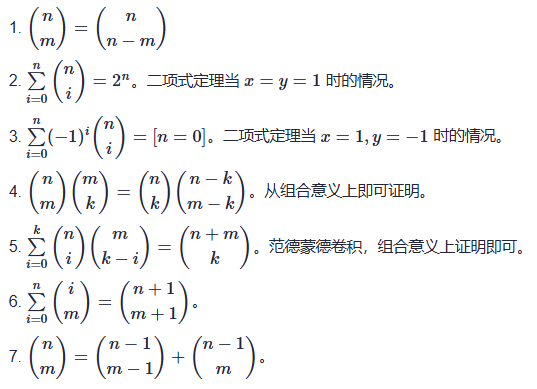
\includegraphics[scale=0.55]{image1.png}
        \caption{组合恒等式}
      \end{figure}
    \end{frame}

  \subsection{二项式系数}
    \begin{frame}{二项式定理}
      \begin{block}{二项式定理}
        \[
        (x+y)^n=\sum\limits_{i=0}^{n}{n \choose i}x^{n-i}y^i
        \]
      \end{block}
      \pause
      \begin{block}{拓展------下降(上升)幂二项式定理}\label{ux62d3ux5c55ux4e0bux964dux4e0aux5347ux5e42ux4e8cux9879ux5f0fux5b9aux7406}
        \[
        \begin{aligned}
        (x+y)^{\underline{n}}=\sum\limits_{i=0}^{n}{n \choose i}x^{\underline{n-i}}y^{\underline{i}} \\
        (x+y)^{\overline{n}}=\sum\limits_{i=0}^{n}{n \choose i}x^{\overline{n-i}}y^{\overline{i}} \\
        \end{aligned}
        \]
      \end{block}
    \end{frame}

    \begin{frame}
      \begin{block}{证明(这里不用数学归纳法进行证明)}
        \[
        \begin{aligned}
        \sum\limits_{i=0}^{n}{n \choose i}x^{\overline{n-i}}y^{\overline{i}}&=\sum\limits_{i=0}^{n}{n! \over (n-i)!i!}x^{\overline{n-i}}y^{\overline{i}} \\\\
        &=\sum\limits_{i=0}^{n}n!{x^{\overline{n-i}}y^{\overline{i}} \over (n-i)!i!} \\
        &=n!\sum\limits_{i=0}^{n}{x \choose i}{y \choose n-i} \\
        (\text{根据范德蒙德卷积})&=n!{x+y \choose n} \\
        &=(x+y)^{\underline{n}} \\
        \end{aligned}
        \]
      \end{block}
      上升幂方法相同。
    \end{frame}

    \begin{frame}{错排}\label{ux9519ux6392}
      \textbf{定义}:一个满足 \(a_i\ne i\) 的序列。
      \textbf{推导式}: \[
      f_n=(n-1)(f_{n-1}+f_{n-2})
      \]
      \pause
      证明

      若当前将 \(1\) 放到位置 \(k(k\ne 1)\),那么 \(k\)
      的放置位置可以分类讨论:
      \begin{enumerate}
      \def\labelenumi{\arabic{enumi}.}
      \item
        \(k\) 放在位置 \(1\) 上,那么还会剩下 \(n-2\) 个数错排,方案数为
        \(f_{n-2}\)。
      \item
        \(k\) 放到某个位置 \(t(t\ne 1)\),那么假设 \(1\) 号位置填上了
        \(P\),则 \(p\ne 1 \land p\ne k\),此时可以考虑一个新序列,把 \(1\)
        去掉,此时方案数为 \(f_{n-1}\)
      \end{enumerate}
    \end{frame}

    \begin{frame}
      \href{https://www.luogu.com.cn/problem/P7438}{例题:P7438 更简单的排列计数}

      设 \(\text{cyc}_\pi\) 将长为 \(n\) 的排列 \(\pi\)
      当成置换时所能分解成的循环个数。给定两个整数 \(n,k\) 和一个 \(k-1\)
      次多项式,对 \(1\leq m\leq n\) 求:

      \[
      \sum\limits_{\pi}F(\text{cyc}_{\pi})
      \]

      其中 \(\pi\) 是长度为 \(m\) 且不存在位置 \(i\) 使得 \(\pi_i=i\) 的排列。
    \end{frame}
    \begin{frame}
      \[
      \begin{aligned}
      \sum\limits_{\pi}F(cyc_\pi)&=\sum\limits_\pi\sum\limits_{i=0}^{k-1}f_i\times cyc_\pi^i \\
      &=\sum\limits_\pi\sum\limits_{i=0}^{k-1}\sum\limits_{j=0}^{i-1} f_i{i \brace j}{cyc_\pi \choose j}j! \\
      &=\sum\limits_{j=0}^{k-1}j!\sum\limits_{i=j}^{k-1}f_i {i \brace j}\sum\limits_\pi{cyc_\pi \choose j}
      \end{aligned}
      \] 
      \pause
      我们发现,\(\sum\limits_{i=j}^{k-1}f_i {i \brace j}\) 与\(\sum\limits_\pi{cyc_\pi \choose j}\) 无关,所以可以将其预处理。

      \(j!,f_i,{i \brace j}\) 都是能够优先处理的。现在考虑\({cyc_\pi \choose j}\) 的处理。
    \end{frame}

    \begin{frame}
      定义函数 \(C_{t,j}\) 为长度为 \(t\) ,环数为 \(j\)
      的排列数,\(P_{t,j}=\sum\limits_{{|\pi |}=t}{cyc_\pi \choose j}\)
      ,通过推导,能够得出: 
      \[
      \begin{aligned}
      C_{t,j}&=(n-1)(C_{t-1,j}+C_{t-2,j-1}) \\
      P_{t,j}&=(n-1)(P_{t-1,j}+P_{t-2,j-1}+P_{t-1,j-1})
      \end{aligned}
      \] 
      \pause
      那么答案即为: 
      \[
      \begin{aligned}
      \sum\limits_{j=0}^{k-1}j!\sum\limits_{i=j}^{k-1}f_i {i \brace j}\sum\limits_{k=1}^nP_{i,j}
      \end{aligned}
      \] 
      其中 \(i\) 的复杂度为 \(O(n)\) ,\(j\) 的复杂度为
      \(O(k)\),总复杂度为 \(O(nk)\),不会超时。
    \end{frame}

  \subsection{容斥原理}
    \begin{frame}{容斥原理}
      对于一个集合 \(S\) 的一部分子集构成的簇 \(P\) 有: \[
      |\bigcup\limits_{T\in P}T|=\sum\limits_{Q \subseteq P}(-1)^{|Q|-1}|\bigcap\limits_{T
      \in Q}T|
      \] 基本容斥原理为高中必学内容,这里对此不过多阐述。
    \end{frame}

    \begin{frame}{鸽巢定理}
      \textbf{原理}:将 \((\sum\limits_{i=1}^{n}p_i)-n+1\) 个东西放入 \(n\)个盒子中,一定存在一个盒子 \(i\),使得第 \(i\) 个盒子至少装了 \(p_i\)个物品。

      证明(反证法)

      \[ \forall x\in \mathbb{N^* } \land 1\le x \le n,a\_i \]
      \pause
      \begin{block}{练习四}\label{ux7ec3ux4e60ux56db}
        有十个数 \(a_1,a_2...a_10\) 满足
        \(\forall_{1\le i\le 10}1\le a_i\le 60\),证明能够从 \(a_i\)
        中挑出两个交为空的子集,使得它们的和相等。
      \end{block}
      \pause
      证明

      两个交为空的子集和相等,所以加上交集后和仍不变,总共有
      \(2^{10}=1024\),但值域仅为 \([0,600]\),故能够选出。
    \end{frame}

    \begin{frame}{鸽巢定理}
      \begin{block}{练习五}\label{ux7ec3ux4e60ux4e94}
      证明一张有超过 \(1\) 个点的简单无向图必定有两点度数相等。
      \end{block}
      \pause
      证明

      考虑分类讨论:

      \begin{enumerate}
        \def\labelenumi{\arabic{enumi}.}
        \item
          有 \(2\) 个度数为 \(0\) 的点,符合条件。
        \item
          有 \(1\) 个度数为 \(0\) 的点,则第 \(n\) 个点需要连 \(n-1\)
          条边,故至少有一个点符合。
        \item
          没有度数为 \(0\) 的点,那么边数的范围为 \([1,n-1]\),所以符合。
      \end{enumerate}
    \end{frame}

    \begin{frame}
      \begin{block}{练习六}\label{ux7ec3ux4e60ux516d}
        证明能从任意 11 个实数中挑选出 4 个数 \(a,b,c,d\) 满足:
        \((ac+bd)^2\geq\frac 1 2(a^2+b^2)(c^2+d^2)\)
      \end{block}
      \pause
      证明
      
      我们令
      \(\overrightarrow x=(a,b),\overrightarrow y=(c,d)\)。原式变为:\(\overrightarrow x \overrightarrow y \ge \frac{\sqrt{2}}{2}\sqrt{|\overrightarrow x||\overrightarrow y|}\)。那么就有:\(\cos<\overrightarrow x,\overrightarrow y>=\frac{\overrightarrow x \overrightarrow y}{\sqrt{|\overrightarrow x||\overrightarrow y|}} \ge \frac{\sqrt{2}}{2}\)
      \textgreater{} 故 \(\overrightarrow x\) 与 \(\overrightarrow y\)
      的夹角为 \(45\) 度。然后我们发现,\(11\) 个实数中必定有至少 \(6\)
      个正数或负数,故我们只需选择正负性相同的 \(4\)
      个数字,这样两条向量一定在同一象限。因为我们有在同一象限的 \(3\)
      条向量,每两条之间最大夹角小于 \(45\) 度。故得证。

    \end{frame}

  \section{二项式反演}
  \subsection{二项式反演}

    \begin{frame}
      \begin{block}{二项式反演}\label{ux4e8cux9879ux5f0fux53cdux6f14}
        \textbf{结论}: 
        \[
        \begin{aligned}
        F(n)&=\sum\limits_{i=m}^{n}{n \choose i}G(i) \\
        G(n)&=\sum\limits_{i=m}^{n}(-1)^{n-i}{n \choose i} F(i) \\
        F(n)&=\sum\limits_{i=m}^{n}{i \choose m}G(i) \\
        G(n)&=\sum\limits_{i=m}^{n}(-1)^{i-m}{i \choose m} F(i) \\
        \end{aligned}
        \]
      \end{block}
    \end{frame}

    \begin{frame}
      \[
      \begin{aligned}
      F(n)=\sum\limits_{i=m}^n\dbinom ni\sum\limits_{j=m}^i(-1)^{i-j}\dbinom ijF(j)=\sum\limits_{j=m}^nF(j)\sum\limits_{i=j}^n\dbinom ni\dbinom ij(-1)^{i-j} \\
      =\sum\limits_{j=m}^nF(j)\sum\limits_{i=j}^n\dbinom nj\dbinom {n-j}{i-j}(-1)^{i-j} \\
      =\sum\limits_{j=m}^n\dbinom nj F(j)\sum\limits_{i=j}^n\dbinom {n-j}{i-j}(-1)^{i-j} \\
      =\sum\limits_{j=m}^n\dbinom nj F(j)\sum\limits_{i=0}^{n-j}\dbinom {n-j}{i}(-1)^{i} \\
      =\sum\limits_{j=m}^n\dbinom nj F(j)[n=j]=F(n)
      \end{aligned}
      \]
      第二种形式证明类似。
    \end{frame}

    \begin{frame}
      \begin{block}{\href{https://www.luogu.com.cn/problem/P10596}{练习七 BZOJ2839
      集合计数(P10596)}}

      有 \(n\)个元素,问有多少种选择若干个子集的方案,使得选出的子集的交集恰好为\(k\)。

      \(0 < k \le n \le 10^6\)
      \end{block}
      \pause
      我们先考虑子集的交集大小至少为 \(i\) 的方案,记为
      \(F(i)\),那么相当于先挑出 \(i\) 个,再从 \(n-i\)
      个中计算出剩余元素的子集的数量即为
      \(2^{n-i}\),然后我们需要在这些剩余子集中的挑选子集方案,即为
      \(2^{2^{n-i}}\),考虑到当剩余子集为空时,方案就为 \(i\) ,舍去,所以可得
      \(F(i)={n \choose i}(2^{2^{n-i}}-1)\)。
    \end{frame}
    \begin{frame}
      然后我们考虑答案函数 \(G(k)\),因为 \(F(i)\)
      在求解时会对所有交集大小大于等于 \(i\) 的情况计数,理想情况下应该计数
      \(1\) 次,但是经过画图可以发现,当我们处理类似 \(G(i+1)\)
      的情况时,其也会对 \(F(i)\) 产生贡献,贡献为
      \({i+1 \choose i}\),所以可以得出结论: 
      \[
      F(i)=\sum\limits_{j=i}^{n}{j \choose i}G(j)
      \] 
      进行二项式反演可得: 
      \[
      \begin{aligned}
      G(k)&=\sum\limits_{i=k}^{n}{i \choose k}(-1)^{i-k}F(i)\\
      &=\sum\limits_{i=k}^{n}(-1)^{i-k}{i \choose k}{n \choose i}(2^{2^{n-i}}-1)
      \end{aligned}
      \]
      现在就可以解决了。
    \end{frame}

    \begin{frame}
      \begin{block}{\href{https://www.luogu.com.cn/problem/P4859}{练习八 BZOJ3622
      已经没有什么好害怕的了(P4859)}}

      有两个序列 \(a_i,b_i\) 保证所有元素互不相同。你需要重排 \(b\)
      序列,使得恰好有 \(k\) 个 \(i\) 满足 \(a_i>b_i\)。,求方案数。

      \(0<k\leq n\leq2000\)。
      \end{block}
      \pause
      先将 \(a\) 序列排序,使其单调上升。

      考虑 \(dp_{i,j}\) 表示考虑前 \(i\) 对数,恰有 \(j\) 对 \(a_i>b_i\)
      ,这样无法转移。

      还是先考虑前 \(i\) 个中至少 \(j\) 对 \(a_i>b_i\),设为
      \(dp_{i,j}\),那么就有 \[
      dp_{i,j}=dp_{i-1,j}+dp_{i-1,j-1}*(cnt(a_i)-j+1)
      \] \(cnt(a_i)\) 表示在当前 \(i\) 位置,有多少个 \(b\) 满足 \(a_i>b\)。
    \end{frame}

    \begin{frame}
      然后设 \(F(i)\) 表示钦定 \(i\) 对符合条件的方案数,\(G(i)\) 表示恰好
      \(i\) 对的方案数。在当前位置,由于钦定 \(i\)
      对符合,所以剩下的数随便排序,就为 \(A_{n-i}^{n-i}=(n-1)!\),就有: 
      \[
      (n-i)!dp_{n,i}=F(i)=\sum\limits_{j=i}^{n}{j \choose i}G(j)
      \] 
      \pause
      反演可得: 
      \[
      \begin{aligned}
      G( k)&=\sum\limits_{i=k}^{n}{i \choose k}(-1)^{i-k}F(i) \\
      &=\sum\limits_{i=k}^{n}{i \choose k}(-1)^{i-k}(n-i)!dp_{n,i}
      \end{aligned}
      \] 然后就能够解决啦。
    \end{frame}

    \begin{frame}
      \begin{block}{\href{https://www.luogu.com.cn/problem/CF997C}{练习九 CF997C Sky Full of
      Stars}}

      有一个 \(n\times n\)
      的矩阵,将其三染色,使得至少有一行或者一列同色,问方案数。

      \(n\leq10^6\)
      \end{block}
      \pause
      我们先钦定有 \(i\) 行 \(j\) 列同色,记为 \(F(i,j)\) 
      \[
      F(i,j)=
      \begin{cases}
      3^{(n-i)n+i}{n \choose i} & j=0 \\
      3^{(n-j)n+j}{n \choose j} & i=0 \\
      3^{(n-i)(n-j)+1}{n \choose i}{n \choose j} & i\ne 0,j\ne 0 \\
      \end{cases}
      \] 
      考虑恰好有 \(i\) 行 \(j\) 列同色,记为 \(G(i,j)\)
      我们需要求至少一行一列,所以可以用 \(全集-G(0,0)\)。
    \end{frame}

    \begin{frame}
      \[
      \begin{aligned}
      &F(x,y)=\sum\limits_{i=x}^{n}\sum\limits_{j=y}^{n}{i \choose x}{j \choose y}G(i,j) \\
      &G(x,y)=\sum\limits_{i=x}^{n}\sum\limits_{j=y}^{n}(-1)^{i+j-x-y}{i \choose x}{j \choose y}F(i,j) \\
      &G(0,0)=3^{n^2}+\sum\limits_{i=1}^{n}(-1)^{n-i}{n \choose i}(F(0,i)+F(i,0))+\sum\limits_{i=1}^{n}\sum\limits_{j=1}^{n}(-1)^{2n-i-j}{n \choose i}{n \choose j}F(i,j) \\
      &G(0,0)=3^{n^2}+\sum\limits_{i=1}^{n}(-1)^{n-i}{n \choose i}(F(0,i)+F(i,0))+\sum\limits_{i=1}^{n}\sum\limits_{j=1}^{n}(-1)^{i+j}{n \choose i}{n \choose j}F(i,j) \\
      \end{aligned}
      \]
      \pause
      将 \(F(i,j)\) 代入原式子。后面那坨东西即为: 
    \end{frame}

    \begin{frame}
      \[
      \begin{aligned}
      &=\sum\limits_{i=1}^{n}\sum\limits_{j=1}^{n}(-1)^{i+j}{n \choose i}{n \choose j}3\times 3^{(n-i)(n-j)} \\
      &=3^{n^2+1}\sum\limits_{i=1}^{n}{n \choose i}(-1)^i3^{-in}\sum\limits_{j=1}^{n}{n \choose j}(-1)^j3^{-jn}3^{ij} \\
      \end{aligned}
      \] 
      现在发现 \(3^{ij}\)是最不好处理的,因为它使得不能使用二项式定理,先考虑这个的处理方法。 
      \[
      \begin{aligned}
      &=3^{n^2+1}\sum\limits_{i=1}^{n}{n \choose i}(-1)^i3^{-in}\sum\limits_{j=1}^{n}{n \choose j}(-1)^j3^{j(i-n)} \\
      &=3^{n^2+1}\sum\limits_{i=1}^{n}{n \choose i}((-1)^i3^{-in}(1-3^{(i-n)})^n-1) \\
      G(0,0)&=3^{n^2}+\sum\limits_{i=1}^{n}(-1)^{n-i}{n \choose i}(F(0,i)+F(i,0))+(-1)^i3^{-in}\sum\limits_{j=1}^{n}{n \choose j}(-1)^j3^{-jn}3^{ij}
      \end{aligned}
      \] 
      现在就可以处理了。
    \end{frame}
    
    \begin{frame}
      \begin{block}{{练习十(第二类斯特林数通项求法)}\label{ux7ec3ux4e60ux5341ux7b2cux4e8cux7c7bux65afux7279ux6797ux6570ux901aux9879ux6c42ux6cd5}}

      记 \({n\brace m}\) 表示把 \(n\) 个不同的物品划分为 \(m\)
      个集合构成簇的方案数(不允许空集)。
      \pause
      
      我们先设 \(F(n,m)={n \brace m}\),\(G(n,m)\)
      表示允许存在空集时的方案数。
      
      \pause
      易得 \(G(n,m)={m^n \over m!}\)。
      
      \pause
      钦定非空集合数,可以有:
      \(G(n,m)=\sum\limits_{i=1}^{m}{m \choose i}F(n,i)。\)
      
      \pause
      进行反演可得:\(F(n,m)=\sum\limits_{i=1}^{m}{m \choose i}(-1)^{m-i}G(n,i)。\)
      
      \pause
      代入可得:\({n\brace m} = f_{n,m}=\sum\limits_{i=1}^m{(-1)^{m-i}\binom mi {i^n \over i!}}=\sum\limits_{i=1}^m{(-1)^{m-i}{i^n \over i!(m-i)!}}\)。
      
      这也是第二类斯特林数的通项公式。
      \end{block}
    \end{frame}


  \section{Lucas 定理}
  \subsection{Lucas 定理}

    \begin{frame}{Lucas 定理}
      Lucas 定理可以用来求大组合数对小模数取模的结果
      \begin{block}{Lucas 定理}
      \[
      {n \choose m}\equiv{{\lfloor {n \over p} \rfloor} \choose {\lfloor {m \over p} \rfloor}}{{n\bmod p} \choose {m \bmod p}}\pmod p
      \]
      \end{block}
      其中 \(p\) 为质数。
    \end{frame}

    \begin{frame}{Lucas 定理的证明}
      证明
      注意到 \({p \choose n}\equiv[n=p \lor n=0]\pmod p\),
      因此 \((a+b)^p\equiv a^p+b^p \pmod p\)。
      对于 \(f(x)=(1-x)^n,f(x)[x^m]={n \choose m}\)。
      我们现在对 \(f(x)\) 做一点变换,
      \pause
      \[
      \begin{aligned}
      f(x)&=(1+x)^n \\
      &=(1+x)^{p\times\lfloor{n \over p}\rfloor}(1+x)^{n \bmod p} \\
      &=((1+x)^p)^{\lfloor{n \over p}\rfloor}(1+x)^{n \bmod p} \\
      \end{aligned}
      \]
      \[
      f(x)\equiv (1+x^p)^{\lfloor{n \over p}\rfloor}(1+x)^{n \bmod p} \pmod p
      \]
      \pause
      所以对于 \(f(x)\),前半部分 \(((1+x)^p)^{\lfloor{n \over p}\rfloor}\)
      一定为 \(p\) 的倍数,后半部分 \((1+x)^{n \bmod p}\) 一定小于 \(p\) ,设
      \(h(x)=(1+x^p)^{\lfloor{n \over p}\rfloor}\) ,
      \(g(x)=(1+x)^{n \bmod p}\)。
    \end{frame}

    \begin{frame}{Lucas 定理的证明}
      \(f(x)[x^m]=h(x)[x^{kp}]\times g(x)[x^{r}] \pmod p\)

      所以就有
      \(m=kp+r\rightarrow k=\lfloor{m \over k}\rfloor,r=m\bmod p\)。

      就可以得出
      \[
      {n \choose m}\equiv{\lfloor {n \over p} \rfloor \choose \lfloor {m \over p} \rfloor}{{n\bmod p}\choose {m \bmod p}}\pmod p
      \]
    \end{frame}

\end{document}